\documentclass{article}
\usepackage{hyperref}
\usepackage{graphicx}
\usepackage{float}
\usepackage{placeins}
\usepackage{rotating}
\hypersetup{
    colorlinks,
    citecolor=black,
    filecolor=black,
    linkcolor=black,
    urlcolor=black
}
\begin{document}
\begin{figure}[t]
			\centering
			
\includegraphics[width=300px]{UP_Logo.jpg}
\end{figure}
\title{NavUp Architectural Design}
\maketitle
		\begin{center}
			\textbf{\newline Team Java} \\
		\end{center}
		
		\begin{flushright} \large
			Dail Nathan Jonker - u13325630 \newline
			Kulani Bamuza - u15008402 \newline
			Yashvir Brijlal - u14387744 \newline
			Bayanda Chakuma - u11283212 \newline
			Xolo Dandashe - u14245681 \newline     
		\end{flushright}
\clearpage
\tableofcontents
	
\clearpage
\section{Specific Requirements}
	\subsection{External Interface Requirements}
		\subsubsection{User Interface}
The UI(user interface) of NavUp will be designed to be user friendly. This is required to make the mobile application easy to use for the user. This will in turn reduce the time it takes the user to get accustomed to the mobile application and it's functionality. The UI will offer the base functionality to both a guest and logged-in user. A guest user will be able to open the application and use the navigation system of NavUP like any other user. It will display the various points of interest and activites as well for guests when they visit campus. Activities that might interest a guest to campus will be highlighted on the map itself. A user will be able to easily log in or register to gain access to further functionality of the system. The UI will provide the user with the necessary tools and information to navigate in and around campus grounds. The user will require valid login details to be able to log in to the system. Certain users will have administrative rights allowing them to edit data of the NavUP system. These users will be adding and removing data as required.

		\subsubsection{Hardware Interface}
The hardware required will have to be in the form of a smartphone/tablet. The system will be designed with the idea of it being mobile. The system will thus be developed on a mobile platform for it to be downloaded as an application to be used on a smartphone or tablet. This will allow the system to be used on the go. Most students are on the move meaning they need hardware that can track and navigate them in real time. The wifi hotspots will be a key feuture when GIS is not being used.

		\subsubsection{Software Interface}
The mobile application itself will be designed to function on the Android and IOS mobile platforms. These platforms have touchscreen capabilities, allowing the user to use the system as any other application on their smartphone. The built in software of each platform allows the system to be compacked, users will be able to easily navigate and search various locations by using the on-board keyboard of the smartphone. GIS and wifi will allow the software to locate there position and navigate a route for students aswell as provide relevent information on the location they are at.

		\subsubsection{Communications Interface}
As stated in the SRS document, the system will be using GIS navigation. It will also make use of wifi-signal strength to determine a user's position depending on the various wifi hotspots on campus. A user will make use of these technologies in various ways, but they need to be connected to the system in some form to gain access to it, this includes mobile data and wifi. Seeing as campus has wifi available to guests and students/staff, this allows for easier communication between the smartphone app and the system itself. This will also help save mobile data for the users when navigating or searching for locations on campus. The system will also communicate to the user in the form of notifications on the application itself and via email when certain tasks are done by the user.
	\subsection{Performance Requirements}
The mobile version of NavUp needs to funtion like any other mobile application. There should not be any indication of delay when moving between interfaces and using the functionality of the application. The only delay that can be acceptible is the connection to the system or determining a user's location. This can be caused by a user's smartphone that has a weak signal/connection to the system. This can also happen when connection is lost or interrupted. The application itself needs to opperate smoothly on any smartphone device that can support it. This means that it needs to be designed with old smartphones in mind, allowing all smartpfone users to use it without any delay. Position needs to be calculated as fast as possible including navigating a path for a user. The end point will be static information saved in the database, this needs to be fetched as quick as possible for the route to be calculated. Unnecessary delay may be frustrating to the user.	
	\subsection{Design Constraints}
The mobile application cannot be too large in size. Users sometimes have limited space left on their smartphone device, this will then require the application to be as small as possible while stil maintaining propper functionality. The static data will be stored on a database along with any user information on a server which will reduce the size drastically. The map itself will be the largest part of the application, so care needs to be taken of what detail and size the map will consist of. The remainder of the apllication must take care not to overstep the size boundry(This will be set at a later stage, most likely in implementation). 
	\subsection{Software System Attributes}
		\subsubsection{Realiability}
		The system itself will never crash or hang, excluding an operating system error. The system will provide alternatives when connection has been lost or when there is a delay when connecting. The system will continue to try and re-connect when connection has been lost.
		\subsubsection{Availability}
		The system will be available to all users that have access to a smartphone or tablet. A web based version will also be available to administrative users at all times.
		\subsubsection{Security}
		The user's information will be kept confidential and will not be used for other purposes than the system itself. Only administrative users will have access to this information. Information like passwords will be encrypted before it is saved on the database.
		\subsubsection{Maintainabilty}
		The code of the system will be modular to allow for future modifications to improve or add on to features. The code itself will be documented and authorship will be added for refrencing purposes. The system itself and the database will be maintained and monitored by the administrative users.
		\subsubsection{Interoperability}
		User devices will communicate with the system, exchanging information required for the functionality of the system. User devices will use this information to display relevant and required data to the user and in turn provide feedback to the system when updates are made.

\section{UML Diagrams}
In this section of the document the various diagrams of the sub-systems will be illustrated. The main diagrams will include a Use Case and Class diagrams. State, Sequence and Activity diagrams may be included to expand on non-trivial functionality.
	\subsection{Users}
	The following Diagrams include a Use Case and Class diagram for the User sub-system:	
	\FloatBarrier	
	\begin{figure}[h]
		\caption{User Use Case Diagram}
		\centering
  		\includegraphics[scale=0.4]{Images/UsersUseCase.png}
	\end{figure}
	\begin{figure}[h]
	\caption{User Class Diagram}
	\centering
  		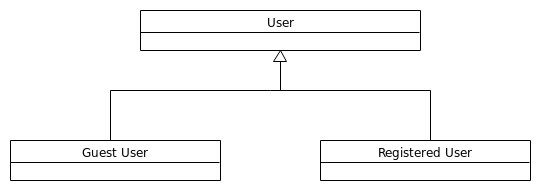
\includegraphics[width=\textwidth]{Images/UserClass.png}
	\end{figure}
	\FloatBarrier
	\subsection{Navigation}
	The following Diagrams include a Use Case, State and Class diagram for the Navigation sub-system:
	\FloatBarrier	
	\begin{figure}[h]
		\caption{Navigation Use Case Diagram}
  		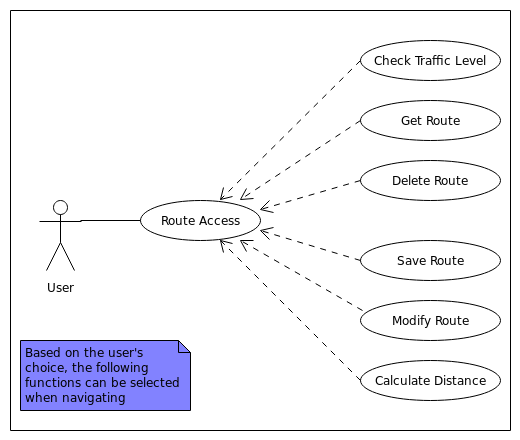
\includegraphics[width=\textwidth]{Images/NavigationUseCase.png}
	\end{figure}
	\begin{figure}[h]
		\caption{Navigation Class Diagram}
  		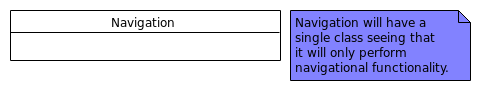
\includegraphics[width=\textwidth]{Images/NavigationClass.png}
	\end{figure}
	\begin{figure}[h]
		\caption{Navigation State Diagram}
  		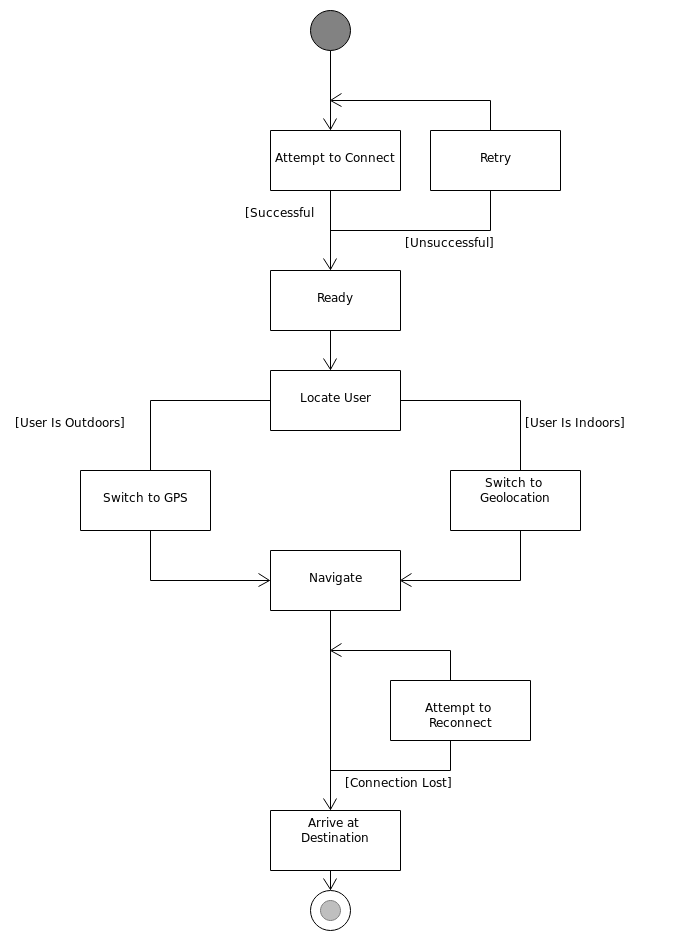
\includegraphics[width=\textwidth]{Images/NavigationState.png}
	\end{figure}
	\FloatBarrier	
	\subsection{Notification}
	The following Diagrams include a Use Case, Sequence and Class diagram for the Notification sub-system:
	\FloatBarrier	
	\begin{figure}[h]
		\caption{Notification Use Case Diagram}
  		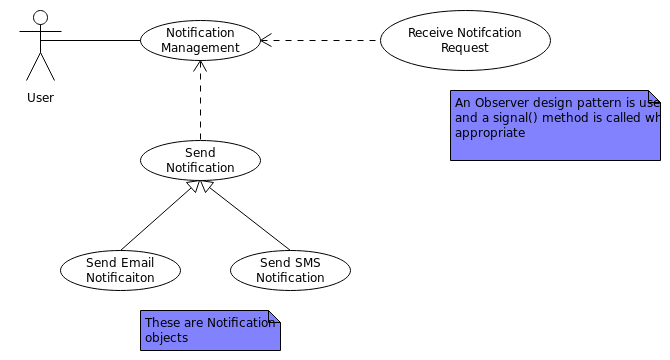
\includegraphics[width=\textwidth]{Images/NotificationUseCase.png}
	\end{figure}
	\begin{sidewaysfigure}[h]
		\caption{Notification Class Diagram}
  		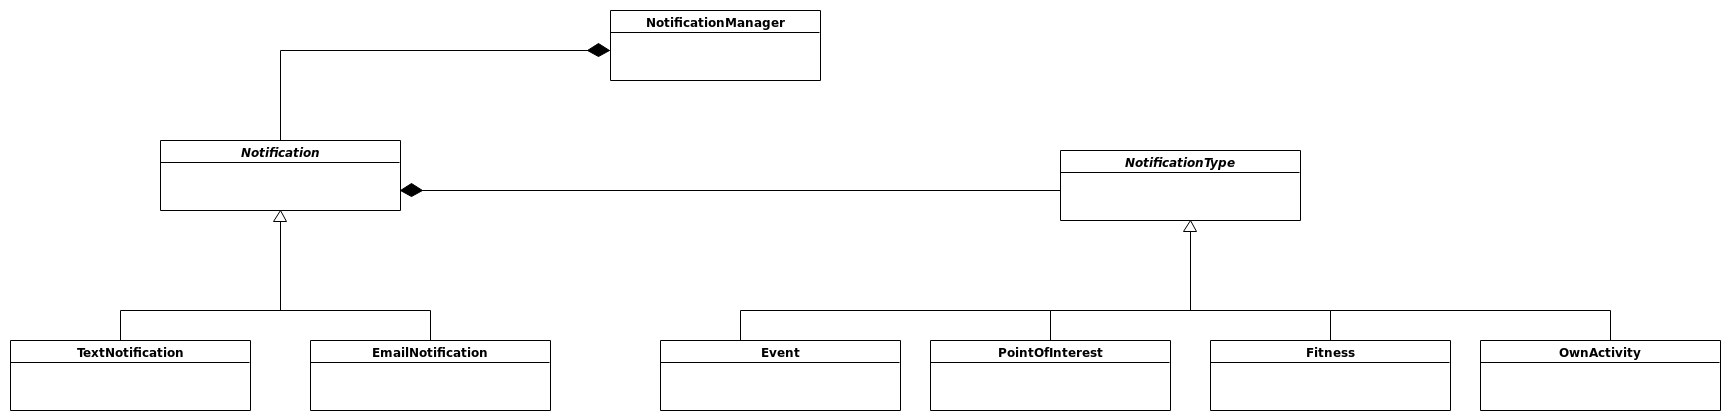
\includegraphics[width=\textwidth]{Images/NotificationClass.png}
	\end{sidewaysfigure}
	\begin{figure}[h]
		\caption{Notification Sequence Diagram}
  		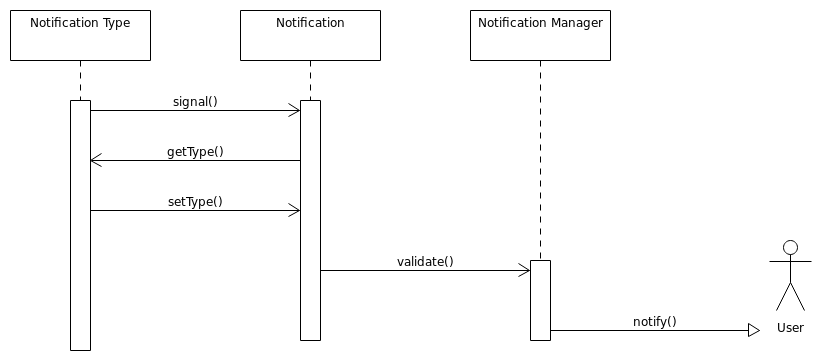
\includegraphics[width=\textwidth]{Images/NotificationSequence.png}
	\end{figure}
	\FloatBarrier	
	\subsection{Points of Interest}
	The following Diagrams include a Use Case and Class diagram for the Points of Interest sub-system:
	\FloatBarrier	
	\begin{figure}[h]
		\caption{Points of Interest Use Case Diagram}
  		\includegraphics[scale=0.4]{Images/POIUseCase.png}
	\end{figure}
	\begin{figure}[h]
		\caption{Points of Interest Class Diagram}
  		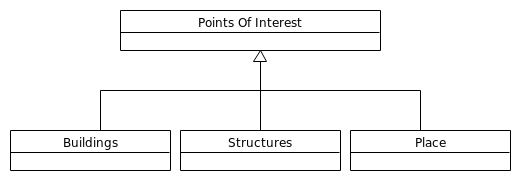
\includegraphics[width=\textwidth]{Images/POIClass.png}
	\end{figure}
	\FloatBarrier
	\clearpage	
\section{Deployment Diagram}
The following Deployment diagram will illustrate the system as a whole, visualizing hardware, platforms and the software that runs on it:
	\FloatBarrier	
	\begin{figure}[h]
		\caption{System(NavUP) Deployment Diagram}
  		\includegraphics[scale=0.4]{Images/Deployment.png}
	\end{figure}
	\FloatBarrier	
	\clearpage

\section{Design Pattern}
The following will explain the various design patterns chosen:
	\FloatBarrier	
	\begin{figure}[h]
		\centering
		\caption{Singleton Design Pattern}
  		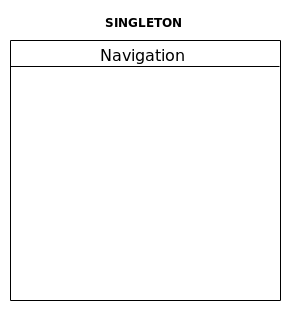
\includegraphics[width=200px]{Images/Singleton.png}
	\end{figure}
	\begin{sidewaysfigure}[h]
		\caption{Facade Design Pattern}
  		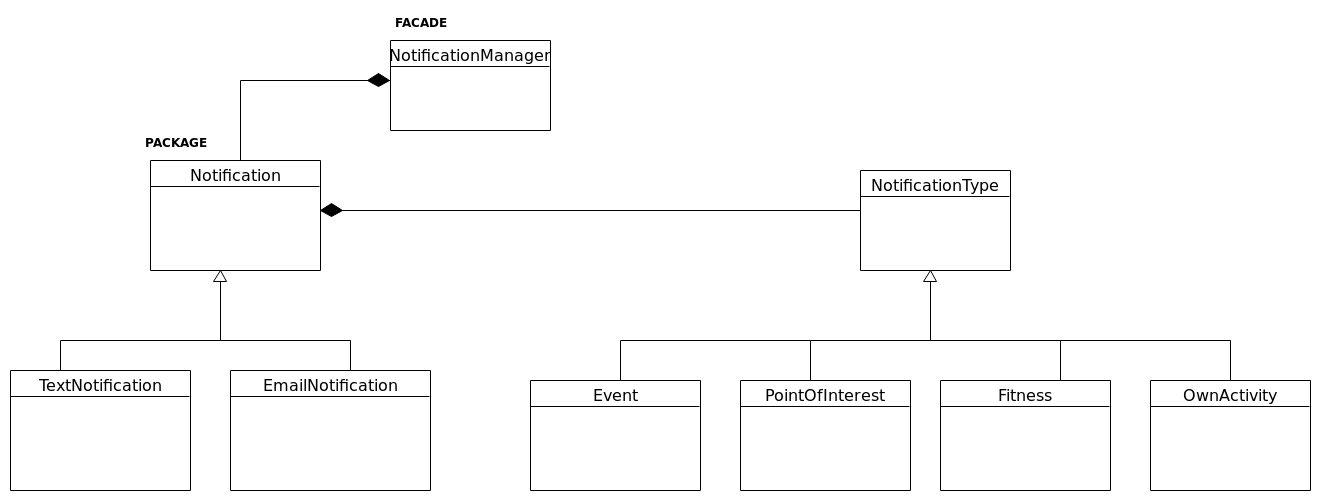
\includegraphics[width=\textwidth]{Images/Facade.png}
	\end{sidewaysfigure}
	\begin{sidewaysfigure}[h]
		\caption{Factory Design Pattern}
  		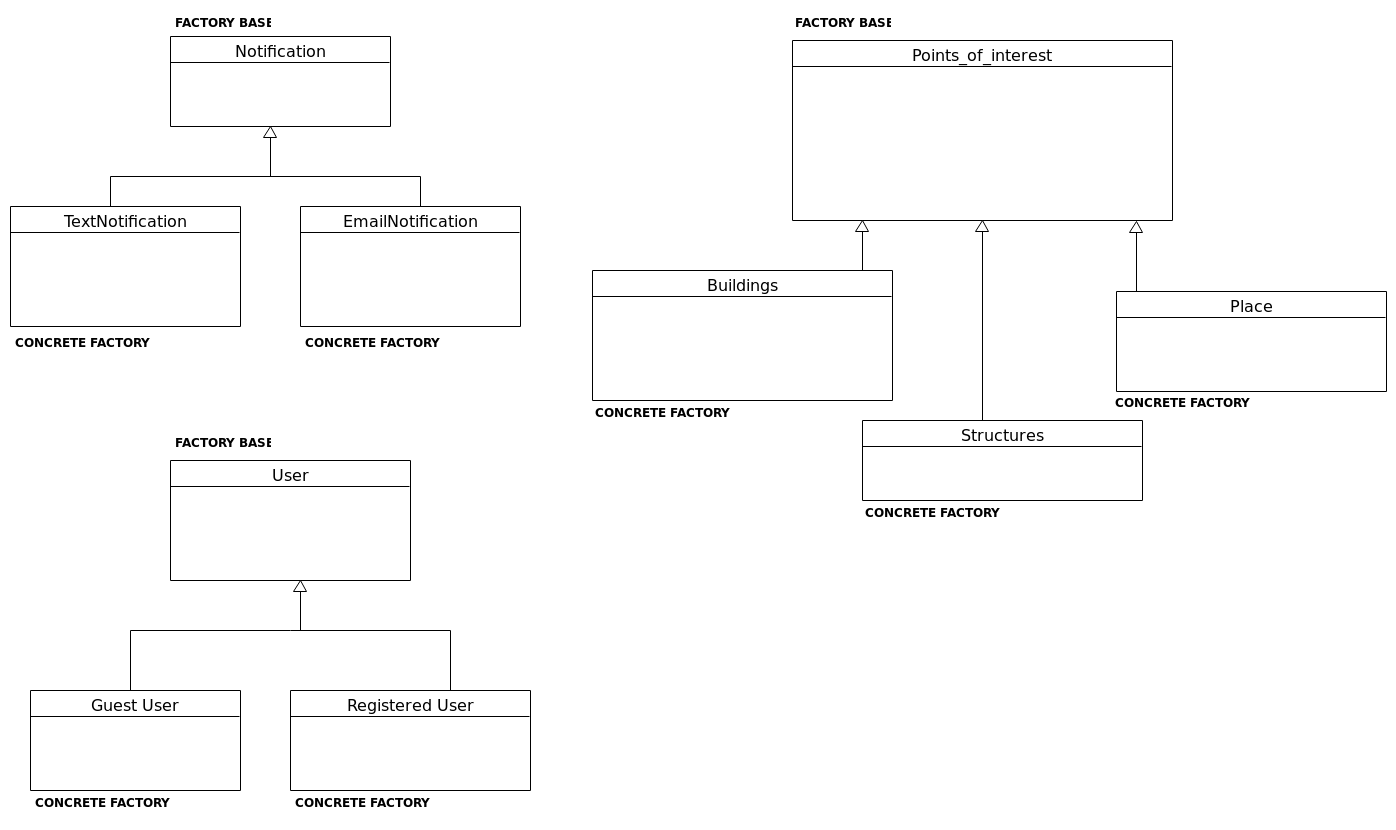
\includegraphics[width=\textwidth]{Images/Factory.png}
	\end{sidewaysfigure}
	\begin{sidewaysfigure}[h]
		\caption{Observer Design Pattern}
  		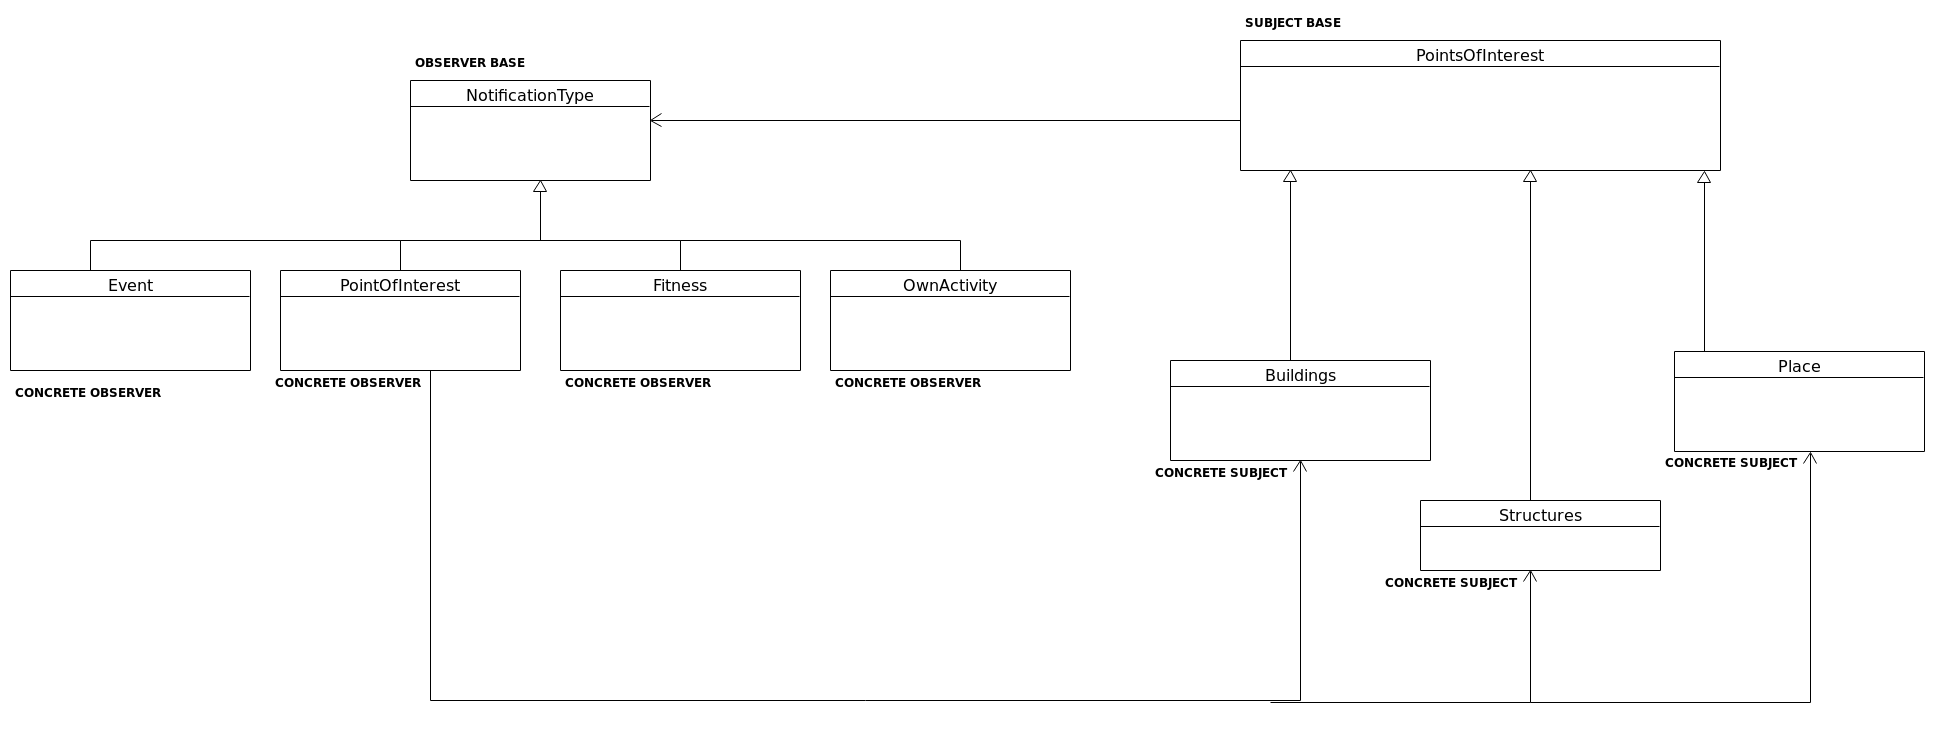
\includegraphics[width=650px]{Images/Observer.png}
	\end{sidewaysfigure}
	\FloatBarrier	

\section{Technologies}
The application makes use of various technologies in order to implement its functionality. These technologies include, but are not limited to, back end programming languages, web design technologies, web development technologies, navigation technologies, networking technologies and database technologies.  The technologies used are based on the implementation designed and specified within this document.  
	\subsection{Platform}
The two most popular mobile platforms by far are Apple and Android.  As such, the system will be implemented on these platforms as to cater to the vast majority within the user base. 
		\begin{itemize}
			\item iOS
			\item Android
		\end{itemize}
	\subsection{Application Programming}
Parts of the system's backend and certain functionality is implemented on the application and not in the largely web based interface.  This requires platform-specific technologies. These technologies were chosen as they are the standard programming language used in their respective environments.
		\begin{itemize}
			\item Swift (iOS)
			\item Java (Android)
		\end{itemize}
	\subsection{Interface}
The system's interface will be largely web based. This is due to the fact that there needs to be real time updates within the interface, constant data retrieval and a persistent internet connection.  Additionally all web technologies are designed in such a way that they can easily integrate with one another thus the system can make use of the various strengths of a particular technology yet not being bound to its limitations.  Additionally, within these technologies some are used for web design, and others web development.  The application's interface is a combination of these two categories:
		\subsubsection{Web Design}
			\begin{itemize}
				\item HTML
				\item CSS
				\item Bootstrap
				\item XML
			\end{itemize}
		\subsubsection{Web Development}
			\begin{itemize}
				\item PHP
				\item Javascript
			\end{itemize}
	\subsection{Database}
Database and data storage is an integral part of the system.  The application heavily makes use of persisted data, be it user information or point of interest information etc.  Thus a large database with multiple tables needs to be maintained.  Given the system requires fast data retrieval, a technology that offers high performance at scale is used.
		\begin{itemize}
			\item MongoDB
		\end{itemize}
	\subsection{Networking}	
The ability to communicate with the various routers around campus is of utmost importance.  The applications requires networking capabiilties in order to ping routers and deduce the user's location.  In order to do this a technology is employed to scan the surrounding routers and ping them.
		\begin{itemize}
			\item Nmap
			\item OAuth2 tokens
item
		\end{itemize}
	\subsection{Navigation}
NavUP is essentially a navigation application.  Specialized technologies are used for this purpose.  The application utilizes these technologies in order to obtain locations, calculate routes and distances, find locations etc.  
		\begin{itemize}
			\item GPS
			\item Google Maps API
		\end{itemize}

\end{document}